\cotefile{85}
\scanpage{58}
% l. 1, in two hands
\margin{(16 p)}hyperpolygônes réguliers.
% archive sheet number: 57
\scanpage{59}
% l. 1
Cas $n=1$, sur corps \inserted{$k$} car. 0, $G_{0}$ fini

% ll. 2–3
\[
\begin{array}{cccl}
\mu_0,&\mu_1,&\beta&\text{invariant}\\[-2pt]
\shortparallel&\shortparallel&\shortparallel&\\
\lambda_0-1&\lambda_1-1&\alpha+2&
\end{array}
\]

% ll. 4–5
1) $\mu_0,\mu_1\ne0$ i.e. $\lambda_0,\lambda_1\ne1$ \quad ($\tau_0,\tau_1$ d'ordre fini)

$\lambda_0,\lambda_1$ racines de l'unité (d'ordre $\underline{\nu}_0,\underline{\nu}_1\unsure{\geqslant|>}2$)

% ll. 6–10
2) $\langle\pi,\pi'\rangle=\underset{\shortparallel\,\inserted{\deleted{\unsure{\beta}}\mu_0\mu_1-\beta}}{\rho}\ne0$ \quad i.e. $\unsure{E|\mathcal E}\simeq V\oplus k\pi$ \qquad On peut se borner : $V$

Système de deux ps. réflexions strictes $\tau_0,\tau_1$ dans $V$, avec conditions de non dégénérescence :

\[
\begin{aligned}
\text{a)}\;&\langle a_0,a'_1\rangle\ne0\\
\text{b)}\;&a_0,a_1\quad\text{lin. indép.}
\end{aligned}
\]

% ll. 11–15
I) La représentation dans $C=\check{\mathbb P}(V)$ admet un div. de degré 2 invariant

Il ne peut être réduit à un pt, car s'il y a une droite \inserted{$\subset V$} \uline{invariante} par $G_0$, il y a une \unsure{suppl|supplém.}, donc $G_0$ est \unsure{comm|commutatif} $\subset k^\times\times k^\times$, absurde.

% ll. 16–21
Donc $V=D\oplus D'$, et pour la $=$ raison que dessus, $D,D'$ ne sont pas invariantes par $\tau_0,\tau_1$ à la fois

\deleted{a) $\tau_0$ invarie $D,D'$, $\tau_1$ \unsure{non}} \inserted{Si $\tau_i$ invarie $D$,} c'est que ou bien $a'_i$ est nul sur $D$, ou bien $a^{\deleted{\unsure{\prime}}}_i\in D$. Dans le premier cas, on aurait $a_i\in D'$, dans le deuxième $a'_i$ nul sur $D'$. Ainsi, OPS $a_i\in D$, $a'_i$ nul sur $D'$, donc
\[
D=ka_i,\quad D'=\operatorname{Ker}a'_i
\]

% ll. 22–26
Considérons alors \deleted{$j\ne i\quad \unsure{0\leq j\leq1}$} \inserted{$j\ne i,\ j\in\{0,1\}$}, alors $\tau_jD\subset D'$, $\tau_jD'\subset D$,
\[
a_i+\underbrace{\langle a_i,a'_j\rangle}_{\deleted{\unsure{\mu_0\beta}}}a_j\in D'
\quad\text{i.e.}\quad
\underbrace{\langle a_i,a'_i\rangle}_{\mu_i}
+\underbrace{\langle a_i,a'_j\rangle\langle a_j,a'_i\rangle}_{\beta}=0
\]
d'où $\beta\ne0$, donc quitte à intervertir $\tau_0,\tau_1$ SPG que $i=0$, $j=1$ \quad $\beta=-\mu_0$. Exprimons aussi $\tau_1D'\subset D$ i.e. $\tau_1^2D\subset D$, $\tau_1^2=\mathrm{id}+(2+\mu_1)a'_1\otimes a_1$
% archive sheet number: 58
\scanpage{60}
% ll. 1–5
On trouve
\[
\begin{aligned}
&a_0+(2+\mu_1)\langle a_0,a'_1\rangle a_1\in D'\qquad\text{i.e.}\\
&\underbrace{\langle a_0,a'_0\rangle}_{\mu_0}+
(2+\mu_1)\underbrace{\langle\deleted{\unsure{a}}a_0,a'_1\rangle
\langle a_1,a'_0\rangle}_{\beta}=0\\
&\text{i.e.}\qquad \mu_0+(2+\mu_1)\beta=0\qquad\text{i.e.}\quad
\deleted{(2+\mu_1)\beta\unsure{=(\text{comme }\beta|(\text{comme }\beta}}\\
&(\text{comme }\mu_0=-\beta)\qquad(1+\mu_1)\beta=0\quad\text{i.e. comme }\beta\ne0,\\
&1+\mu_1=0\quad\text{i.e.}\quad
\deleted{\mu_1=-1\quad\text{i.e.}\quad\lambda_1-1=}\quad
\lambda_1=0,\quad\text{absurde.}
\end{aligned}
\]

% ll. 6–10
Ainsi $\tau_0,\tau_1$ échangent $D_0,D_1$. Prouvons \deleted{\unsure{maintenant}} \inserted{que} $\mu_0=\mu_1=-2$, i.e. $\lambda_0=\lambda_1=-1$, i.e. $\tau_0,\tau_1$ \uline{d'ordre 2} --- i.e. qu'on est dans le cas des polygônes réguliers ordinaires. \deleted{\unsure{Par ce qui précède|Pour ce qui précède}, on aura} \inserted{Prenons coordonnées adaptées :} $D,D'$

\[
\deleted{\unsure{\tau_0\tau_1|\text{Notons}}}\quad
\deleted{D=ka_0,\quad D'=ka_1\quad\text{donc}}
\]

% ll. 11–14
$e_0\in D,\quad e_1=\tau_0e_0$, on aura, si $\tau_0e_1=\zeta e_0$, $\tau_1e_0=\eta e_1$ \inserted{$\tau_1e_1=\xi e_0$}
\[
\tau_0=\begin{pmatrix}0&\zeta\\1&0\end{pmatrix},\quad
\tau_1=\begin{pmatrix}0&\xi\\\eta&0\end{pmatrix}
\]
équations aux valeurs propres
\[
\lambda^2+\zeta=0,\quad\lambda^2+\xi\eta=0
\]
% ll. 15–17
et comme cette équation a la \deleted{\unsure{val. p.}} solution 1, on doit avoir l'autre valeur propre $\lambda_0$ (resp. $\lambda_1$) égale à $-1$\quad O.K.

\begin{center}\rule{1.1cm}{0.3pt}\end{center}

% ll. 18–24
II) Il n'y a pas dans $C=\check{\mathbb P}(V)$ de div. de degré 2 invariant.

Alors on sait que l'image de $G_{0}$ dans $\operatorname{Aut}(C)\simeq \operatorname{GP}(1,k)$ est un des trois groupes $\unsure{\mathcal A|\mathfrak A}_4\subset \unsure{\mathfrak S|\mathscr S}_4,\ \mathcal A_5$. Considérons leurs images inverses dans $\operatorname{SL}(V)$, $\widetilde{\mathcal A}_4\subset\widetilde{\mathfrak S}_4,\ \widetilde{\mathcal A}_5$, \inserted{soit $\widetilde G_0$.} Alors on a donc
\[
G_0\subset\widetilde G_0\cdot\underbrace{k^\times}_{\text{homothéties}}
\]
% archive sheet number: 59
\scanpage{61}
% ll. 1–4
Notons que, si $\unsure{Z_i|z_i}$ \inserted{$\subset\operatorname{GL}(V)$} est le groupe engendré par $\tau_i$, on a $Z_i\cap k^\times=1$ donc $Z_i\hookrightarrow\operatorname{Aut}(C)$, donc $\nu_i$ prend une des valeurs $2,3,4,5$
\[
2\leq\nu_0,\nu_1\leq5
\]

% ll. 5–8
\deleted{Il faut} Plus gén., \deleted{les valeurs propres des \unsure{$\tau_i$ engendrant}} \inserted{pour tte ps. réfl. \inserted{stricte} de $G_{0}$, son} \deleted{\unsure{partic.} des groupes engendrés par} ordre $\nu$ est comprise entre 2 et 5 \ldots
% archive sheet number: 60
\scanpage{62}
% ll. 1–3, top and its right-hand gloss
\[
\begin{aligned}
\unsure{\beta_0|\beta_{\bullet}}:=\beta&=c\,\frac{\mu_0}{\overline{\mu}_1}
=c\,\frac{\lambda_0-1}{\overline{\lambda}_{\unsure{1|0}}-1}
=c\,\frac{(\lambda_0-1)(\lambda_1-1)}{(K_1-1)}
=\zeta(\lambda_0-1)(\lambda_1-1)\\
&\hspace{6cm}=\zeta\mu_0\mu_1
\end{aligned}
\]
\margin{$\deleted{\unsure{\xi}}\zeta=\dfrac{c}{K_1-1}\in\mathbb R$\\
$K_i=\operatorname{Tr}_{\mathbb C/\mathbb R}\lambda_i=\lambda_i+\overline{\lambda_i}$\\
$\hfill=\lambda_i+\lambda_i^{-1}$\\
$(\lambda_i\overline{\lambda_i}=1)$\\
\uline{NB} $\det\tau_0\tau_1=\lambda_0\lambda_1$\\
$\operatorname{Tr}\tau_0\unsure{t_1|\tau_1}=$}

% ll. 4–7
$\zeta$ satisfait à l'équation
\[
\frac{(\lambda_0-1)^2(\lambda_1-1)^2}{\lambda_0\lambda_1}
\left(\zeta^2+2\frac{\lambda_0+\lambda_1}{(\lambda_0-1)(\lambda_1-1)}\zeta
+\frac{\lambda_0^2+\lambda_1^2}{(\lambda_0-1)^2(\lambda_1-1)^2}\right)
=K\in\{-2,-1,0,\alpha,\alpha'\}
\]
qui exprime que $\tau_0^{C}\tau_1^C$ est d'ordre 2, 3, 4 ou 5.

$[u=\tau_0\tau_1$ a comme trace $\lambda_0+\lambda_1+\beta$, comme déterminant $\lambda_0\lambda_1]$, et $K=K(u)=\dfrac{(\operatorname{Tr}u)^2}{\det u}-2$

% ll. 8–10
\uline{NB} Si $\lambda=\exp i\theta$, $\lambda'=\exp i\theta'$, alors $\lvert\lambda+\lambda'\rvert=2\left|\cos\bigl(\frac{\theta'-\theta}{2}\bigr)\right|$, $\lvert\lambda^2+\lambda'{}^2\rvert=2\unsure{\cos|\lvert\cos}(\theta'-\theta)$
\[
\begin{aligned}
|\lambda-1|^2&=2-K(\lambda)\qquad K(\lambda)=\operatorname{Tr}_{\mathbb C/\mathbb R}\lambda=2\cos\theta\\
|\lambda-1|&=2\left|\sin\frac{\theta}{2}\right|
\end{aligned}
\]

% ll. 11–12
\[
\left\{\begin{aligned}
2\frac{\lambda+\lambda'}{(\lambda-1)(\lambda'-1)}
&=-\frac{\deleted{4}\cos\frac{\theta'-\theta}{2}}{\deleted{4}\sin\frac\theta2\sin\frac{\theta'}2}\\
\deleted{\unsure{2}}\frac{\lambda_{\unsure{0}}^2+\lambda'{}^2}{(\lambda-1)^2(\lambda'-1)^2}
&=\frac{2\cos(\theta'-\theta)}{16\sin^2\frac\theta2\sin^2\frac{\theta'}2}
=\frac{1}{\deleted{\unsure{4}}8}\frac{\cos(\theta'-\theta)}{\sin^2\frac\theta2\sin^2\frac{\theta'}2}
\end{aligned}\right.
\]
\margin{$\dfrac{(\lambda_0-1)^2(\lambda_1-1)^2}{\lambda_0\lambda_1}=16\sin^2\!\frac{\theta_0}2\sin^2\!\frac{\theta_1}2$\\
$0<\theta_0,\theta_1\leq\pi$}

% ll. 13–16
\[
\begin{aligned}
\zeta^2&-\frac{\cos\frac{\theta_1-\theta_0}2}{\sin\frac{\theta_0}2\sin\frac{\theta_1}2}\zeta+
\frac{1}{\deleted{\unsure{8}}16}\left(
\frac{\deleted{\unsure{2}}2\cos(\theta_1-\theta_0)-K}
{\sin^2\frac{\theta_0}2\sin^2\frac{\theta_1}2}
\deleted{\unsure{-\frac{K}{16\sin^2\frac{\theta_0}2\sin^2\frac{\theta_1}2}}}\right)=0\\
\Delta(K)&=\frac12\frac{\deleted{\cos\frac{\theta_1-\theta_0}2}}{\sin^2\frac{\theta_0}2\sin^2\frac{\theta_1}2}
\left[\underbrace{2\cos^2\frac{\theta_1-\theta_0}2-\cos\left(\frac{\theta_1-\theta_0}{\deleted{\unsure{2}}}\right)}_{1}+
\frac{\deleted{\unsure{2}}1}{2}K\right]\\
&=\deleted{\unsure{\frac{2+K/2}{2\sin^2\frac{\theta_0}2\sin^2\frac{\theta_1}2}}}
=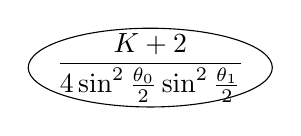
\begin{tikzpicture}[baseline=(x.base)]\node[inner sep=1pt](x){$\displaystyle\frac{K+2}{4\sin^2\frac{\theta_0}2\sin^2\frac{\theta_1}2}$};\draw (x.center) ellipse (1.55cm and .50cm);\end{tikzpicture}
=\ \geqslant0\\
&\hspace{6cm}=\frac{\cos^2\frac\theta2}{\sin^2\frac{\theta_0}2\sin^2\frac{\theta_1}2}
\end{aligned}
\]
\margin{$K+2=2(1+\cos\theta)$\\ $=4\cos^2\frac{\theta}{2}$}
% margin note written sideways
\margin{\rotatebox{90}{\scriptsize $\displaystyle
\zeta=\frac12\left[\frac{\cos\frac{\theta_1-\theta_0}2}{\sin\frac{\theta_0}2\sin\frac{\theta_1}2}
\pm\frac{\deleted{\unsure{\sqrt{K+2}}}\cos\frac\theta2}{\deleted{2}\sin\frac{\theta_0}2\sin\frac{\theta_1}2}\right]
=\frac{1}{\unsure{2}\sin\frac{\theta_0}2\sin\frac{\theta_1}2}
\left[\deleted{\unsure{2}}\cos\frac{\theta_1-\theta_0}2\pm
\deleted{\unsure{\sqrt{K+2}}}\cos\frac\theta2\right]$}}

% ll. 17–20
\deleted{\unsure{Alors} \illegible{2} $\unsure{K+2}$ \unsure{jamais nul} $(\unsure{K+2-\frac18K})$}

N'est nul que si $K=-2$ i.e. $\tau_0^C\tau_1^C$ est d'ordre 2. auquel cas l'unique solution est
\[
\boxed{\zeta=\frac{\cos\frac{\theta_1-\theta_0}2}{2\sin\frac{\theta_0}2\sin\frac{\theta_1}2}}
\]
suivant les valeurs de $\lambda_i=\exp 2i\pi/\nu_i$\quad $2\leq\nu_i\leq5$

Ceci fait $\deleted{16}\inserted{=15}$ possibilités. (en excluant $\nu_0=\nu_1=2$)
% archive sheet number: 61
\scanpage{63}
% ll. 1–4
Pour chacun des \inserted{quatre autres} cas $K=-1,0,\alpha,\alpha'$, ceci fait deux autres possibilités, ce qui fait a priori encore $8\cdot15=120$ possibilités --- mais il faut en exclure un bon paquet \ldots !

% ll. 5–9
Principes et critères d'élimination

a) la condition
\[
0<\zeta<1
\]
exprimant que la forme \deleted{\unsure{sesq.}} hermitienne inv. est définie

% ll. 10–16
b) la condition que \inserted{(le $=$)} $\zeta$ satisfasse des équations analogues quand on change $\theta_0$ en $\deleted{\unsure{k}}i\theta_0$ ($i\not\equiv0\ (\nu_0)$) et $\theta_1$ en $j\theta_1$ ($j\not\equiv0\ (\nu_1)$), quitte à changer $K_{\unsure{*}}$ dans $\{\unsure{2|-2},-1,0,\alpha,\alpha'\}$ --- i.e. que l'ens. des valeurs prises par
\[
16\sin^2\frac{\theta}{2}\sin^2\frac{\theta'}{2}
\left(\zeta^2-\frac{\cos\frac{\theta'-\theta}{2}}{\sin\frac{\deleted{\unsure{\theta_0}}\theta}{2}\sin\frac{\deleted{\unsure{\theta_1}}\theta'}{2}}\zeta+
\frac18\frac{\cos(\theta'-\theta)}{\sin^2\frac{\theta}{2}\sin^2\frac{\theta'}{2}}\right)
\]
pour $\theta=i\theta_0,\ \theta'=j\theta_1$ $(i\not\equiv0\ (\nu_0),\ \theta'\not\equiv0\ (\nu_1))$ est contenu dans $\{-2,-1,0,\alpha,\alpha'\}$ \ldots

\begin{center}\tikz\draw (0,0)--(1.4,0)--(.55,-.04).. controls (1.5,-.08) and (.9,-.15)..(1.09,-.35)--(1.16,-.47);\end{center}
% ll. 17–25
L'analyse géométrique via ``\unsure{syst. de Schwartz|syst. de Schwarz}'' montre que la \uline{situation projective} (dans $C=\check{\mathbb P}(V)$) est déterminée mod iso, par la connaissance  des $K_0,K_1$ et $K$ \deleted{\unsure{à}} (que fixent les \deleted{\unsure{trois} $K_0,K_1$} classes de conjugaison de $\tau_0^{C},\tau_1^C$ et $(\tau_0^C\tau_1^C)^{-1}$ (ou $\tau_0^C\tau_1^C$) dans \deleted{D'autre part, pour} $G=\text{\uline{Aut}}(X)$, ou ce qui revient au $=$, dans le groupe \unsure{pythagoricien} $H$ qu'ils engendrent (mod $\operatorname{Aut}(H)$ dans le cas tétraédral, pas mod $\operatorname{Int}(H)$))
% archive sheet number: 62
\scanpage{64}
% ll. 1–8
D'autre part, pour une situation projective donnée, il y a 4 choix de situations hyperpolygônales à lui donner naissance (suivant le choix d'un des deux pts fixe pour $\tau_0$, et pour $\tau_1$) on passe d'une telle situation \unsure{(numérique|(correspondante|hyperpolygonale} : $\lambda_0,\lambda_1,\ \beta=\zeta(\lambda_0-1)(\lambda_1-1)$ à une autre en remplaçant $\tau_0$ par $\frac{1}{\lambda_0}\tau_0$, ou $\tau_1$ par $\frac{1}{\lambda_1}\tau_1$, ou l'un et l'autre à la fois ---

% ll. 9–14
ce qui ne change pas $K_0,K_1,K'$ car $\tau_0,\tau_1$ et $\tau_0\tau_1$ sont multipliés chacun par un scalaire. \deleted{Donc en principe} Mais ces op. remplacent $(\lambda_0,\lambda_1)$ par $(\lambda_0^{-1},\lambda_1)$ resp $(\lambda_0,\lambda_1^{-1})$ resp $(\lambda_0^{-1},\lambda_1^{\unsure{-|-1}})$ qui \deleted{sont déjà différentes} donnent \inserted{``en général''} \unsure{quadruplement|4 systèmes|un système} de valeurs diff.,

% ll. 15–19
\deleted{tandis que les valeurs correspondantes de $\beta^{\unsure{=}}$, qui ne prend \deleted{au plus} \inserted{a priori} que 2 val. possible, d'après l'équ. donnée plus haut sur $\beta$}
--- ``en général'' signifiant que $\nu_0$ et $\nu_1$ sont $\ne2$, i.e. $\lambda_0,\lambda_1\ne-1$ (i.e. $\mu_0,\mu_1\ne-2$).

% ll. 20–22
Dans ce cas, il s'ensuit donc que pour \deleted{les (2 solutions éventuelles} \inserted{$\lambda_0,\lambda_1$ et $K$ fixés, \deleted{\unsure{quand}} $K\ne-2$} \unsure{NB.} l'équation en $\zeta$ a a priori 2 soln
% archive sheet number: 63
\scanpage{65}
% upper synoptic diagram; read branches from the common middle object
\diagram{\begin{tikzcd}[ampersand replacement=\&,row sep=small,column sep=small]
\parbox{5.4cm}{polygones pythagoriciens\\ \deleted{\unsure{on}}}\arrow[d,leftright] \& \\
\parbox{5.4cm}{\deleted{\uline{certains}} $(\underline{\lambda_0},\underline{\lambda_1},\beta=\underline{\zeta}(\lambda_0-1)(\lambda_1-1)$}
\arrow[d,leftright] \& \\
\parbox{5.4cm}{\uline{\unsure{certains}} couples de 2 ps. réfl. $\tau_0,\tau_1$ dans \inserted{plan} vectoriel $V$ (épinglé par deux vecteurs $a_0\in V^{\tau_0}\ldots$) : conditions de non dég. et d'engendrer d'un groupe fini \ldots}
\arrow[r,leftright] \&
\left\{\parbox{4.6cm}{\deleted{certains \unsure{couples|pythag.}} \inserted{couples} pythagoriciens $(\tau_0^{C},\tau_1^C)$ dans plan proj. $+\,a_0$ point fixe de $\tau_0^C$, $a_1$ pt fixe de $\tau_1^C$}\right.
\arrow[d,leftright]\\
\&\parbox{4.6cm}{\(\left.\begin{array}{c}\text{Ceci décrit}\\\text{la situation}\\\text{pyth. }\text{\uline{projective}}\end{array}\right\}\) donnée des $K_0,K_1,K$ adm.\\ $+\,a_0,a_1$ ds le syst. défini par $K_0,K_1,K$}
\end{tikzcd}}

% small incidence sketch under the left branch
\diagram{\begin{tikzcd}[ampersand replacement=\&,column sep=small,row sep=small]
V\&L_0\arrow[d,dash]\arrow[dr,dash]\&L_1\arrow[d,dash]\\
\&L'_0\&L'_1
\end{tikzcd}}

% middle left
Si $K_i$ fixé, $\lambda_i$ s'en déduit comme \uline{une} des deux solutions de
\[
\lambda_i^2\unsure{-|+}K_i\lambda_i+1=0
\]
le choix des $\deleted{\unsure{K_i}}\lambda_i$ \uline{équivaut}, \deleted{au choix} \inserted{pour} $\lambda_i\ne-1$ i.e. $K_i\ne-2$ i.e. $\nu_i\ne2$, au choix des $a_i$. \deleted{\unsure{en dehors}} Si par contre $\nu_i=2$ i.e. $\lambda_i=-1$ i.e. $K_{\unsure{i|1}}=\unsure{2|-2}$,
\begin{center}\rule{.8\linewidth}{.3pt}\end{center}

% lower working, written upside down; in its own reading order
\[
\left\{\begin{aligned}
\rho(\unsure{\cdot}e_0)&=\deleted{\unsure{e_1|e_0}}\quad\unsure{\varphi|\rho}(e_1)=-e_1\\
\rho'(\unsure{c|e}_0)&=\unsure{\cdot}
\end{aligned}\right.
\]
\[
\begin{aligned}
(\varepsilon_1,\varepsilon_2)^{\deleted{\unsure{2}}}&=g&
g^{\unsure{2|\prime}}&=\mathrm{id}&g'{}^2&=\mathrm{id}&g''{}^2&=\mathrm{id}\\
(\deleted{\unsure{\varepsilon}}\varepsilon'_1,\varepsilon'_2)&=g'&
gg'&=?&g'g''&=?\\
(\varepsilon_3,\varepsilon'_3)&=g''&gg'g''&=
\end{aligned}
\]
\figure{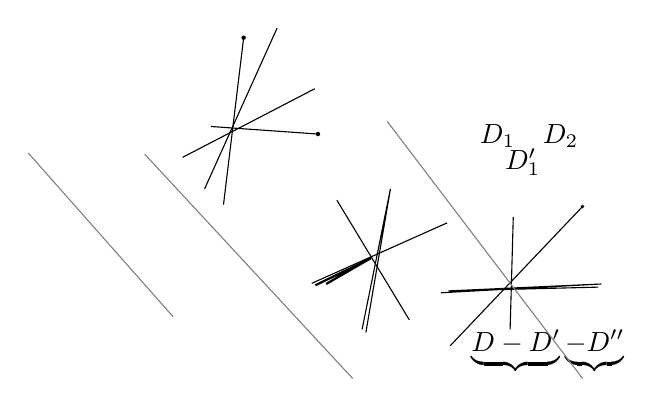
\begin{tikzpicture}[x=.8cm,y=.8cm]
\begin{scope}[shift={(0,2.0)}]
\draw (-.2,-1.2)--(.12,1.45); \fill (.12,1.45) circle (.035);
\draw (-.5,-.95)--(.65,1.6); \draw (-.85,-.45)--(1.25,.64);
\draw (-.4,.04)--(1.3,-.08); \fill (1.3,-.08) circle (.035);
\end{scope}
\begin{scope}[shift={(2.2,-.05)}]
\draw (-.2,-1.13)--(.25,1.1)--(-.14,-1.18);
\draw (-.6,.92)--(.55,-.98); \draw (-1.0,-.40)--(1.15,.56);
\draw[thick] (-.94,-.43)--(-.06,0)--(-.77,-.41);
\end{scope}
\begin{scope}[shift={(4.35,-.55)}]
\draw (-1.1,-.05)--(1.45,.09)--(-.98,-.02)--(1.4,.04);
\draw (0,-.63)--(.05,1.15); \draw (-.95,-.89)--(1.15,1.32);
\fill (1.15,1.32) circle (.03);
\node[above] at (.3,2.1){$D_1\quad D_2$};
\node[above] at (.2,1.65){$D'_1$};
\node[below] at (.6,-.48){$\underbrace{D-D'}\underbrace{-D''}$};
\end{scope}
\draw[thin,gray] (-3.3,1.62)--(-1.0,-.98);
\draw[thin,gray] (-1.45,1.60)--(1.85,-1.96);
\draw[thin,gray] (2.4,2.12)--(5.5,-1.96);
\end{tikzpicture}}
\[
\begin{aligned}
\lambda_0&=\varphi_0^2=(s_0+ic_0)^2=\deleted{\unsure{2}}\underbrace{s_0^2-c_0^2}_{\deleted{\unsure{C}}C_0}+2is_0c_0\\
&&&\hspace{4.5cm}{}+iS_0\\
\lambda_1&=\varphi_1^2=\\
\lambda_0&
\end{aligned}
\]
% archive sheet number: 64
\scanpage{66}
% ll. 1–8
\deleted{Donc le choix} (ce qui ne \unsure{;} peut être le cas que pour un seul des entiers $i=0,1$) alors la donnée de $(\lambda_0,\lambda_1,K)$ ne détermine pas la classe d'iso \unsure{du|de l'|des} hyperpolygône pythagoricien, i.e. ne détermine pas $\zeta$

% ll. 9–12
\uline{En résumé}

a) Pour \diagram{\begin{tikzcd}[ampersand replacement=\&,row sep=.6em,column sep=.18em]
(\lambda_0,\arrow[d,leftright] \& \lambda_1,\arrow[d] \& K)\\
K_0 \& K_1 \&
\end{tikzcd}} admissible \inserted{(du pt de vue projectif)}, \uuline{si} $K_0,K_1\ne-2$ i.e. $\lambda_0,\lambda_1\ne-1$ i.e. $\nu_0,\nu_1\ne2$ il y a un \inserted{et un} seul hyperpolygône associé (mod iso) i.e. un et un seul $\zeta$ correspondant. Si $K=-2$, \inserted{i.e. $\nu=2$,} il est donc donné \deleted{par} \inserted{comme l'unique solution de} l'équation en $\zeta$ ; si $K\ne\unsure{-}2$ parmi les 2 solutions de cette équation, une seule convient pour \inserted{définir} un hyperpolygône pythagoricien. [Comment les distinguer ? Si on travaille dans $\mathbb C$, on peut songer à la condition $0<\zeta<1$ --- ]

% ll. 19–25
b) Par contre si $K_0$ ou $K_1=-2$ i.e. $\lambda_0$ ou $\lambda_1=-1$, \inserted{i.e. $\nu_0$ ou $\nu_{\unsure{1|i}}=2$} alors alors pour $(\lambda_0,\lambda_1,K)$ admissible \inserted{(projectivem.)} donné, il y a \uline{deux} hyperpolygônes non iso qui lui correspondent, correspondant donc aux 2 solutions distinctes $\zeta$ de (E) [NB on sait \inserted{par ailleurs} que l'on aura alors $K=-2$ i.e. que l'on aura bien 2 racines distinctes].

% ll. 26–27
Il n'est donc pas vrai que $\nu_0,\nu_1,\nu$ déterminent la classe d'iso. d'un hyperpolygône, \unsure{$=$|même|---} la.
% archive sheet number: 65
\scanpage{67}
% ll. 1–3
on normalise \inserted{$\lambda_0,\lambda_1$} par le choix de racines primitives $3^{\mathrm e},4^{\mathrm e}$ et $5^{\mathrm e}$ de $1$ (par exemple $\exp 2i\pi/\nu$ quand on est sur $\mathbb C$), et ceci pour deux raisons :

% ll. 4–10
1) Cas où $\lambda_0$ ou $\lambda_1$ \unsure{estt|est} égal à $-1$, i.e. $\nu_0$ ou $\nu_1$ égal 2 --- cela introduit (pour $K$ déjà fixé) une ambiguïté d'ordre 2 :

\diagram{$\begin{array}{l@{\quad}l@{\quad}l}
\text{Cas}&(3,2,3)\quad(2,3,3)&(\inserted{\text{cas}}\ \text{tétraédraux})\\
&(3,2,4)(2,4,3)(2,3,4)(4,2,3)&(\text{octaédraux})\\
&\left\{\begin{array}{l}(3,2,\underline{5})(2,5,3)(2,3,\underline{5})(5,2,3)\\
(5,2,5')(2,5,5')\end{array}\right.&\text{(icosaédraux}
\end{array}$}

% ll. 11–14
2) Cas où $\nu=5$, et où on peut avoir le choix entre $K=\alpha$ et $K=\alpha'$ (cas icosaédral)
\[
\begin{aligned}
&(3,2,5)(2,3,5)\qquad\text{(qui figurent déjà ds liste 1)}\\
&[(3,2,5')\ (2,3,5')]
\end{aligned}
\]
\deleted{\unsure{Si}}

% ll. 15–22
Finalement, compte tenu du choix des racines primitives $3^\circ\ 4^\circ$ et $5^\circ$ de $1$ pour normaliser $\lambda_0,\lambda_1$, on trouve les possibilités suivantes --- où on souligne les possibilités numériques qui donnent lieu à \uline{deux} hyperpolygônes, en interprétant comme d'habitude $5,5'$ comme signifiant $K=\alpha$ resp. $K=\alpha'$ :
% archive sheet number: 66
\scanpage{68}
% upper table, counts in parentheses are placed beneath the triples
\uline{Cas tétraédraux}
\diagram{$\begin{array}{c@{\quad}lll}
&\underset{(4)}{(3,3,2)}&\underset{(2)}{\underline{(3,2,3)}}&\underset{(2)}{\underline{(2,3,3)}}\\
6&\underset{(4)}{(3,3,3)}
\end{array}$}

\uline{Cas octaédraux}
\diagram{\scriptsize\setlength{\arraycolsep}{2pt}$\begin{array}{c@{\quad}llllll}
&\underset{(4)}{(4,3,2)}&\underset{(2)}{\underline{(3,2,4)}}&\underset{(2)}{\underline{(2,4,3)}}&
\underset{(2)}{\underline{(2,3,4)}}&\underset{(4)}{(3,4,2)}&\underset{(2)}{\underline{(4,2,3)}}\\
13&\underset{(4)}{(4,4,3)}&\underset{(4)}{(4,\deleted{\unsure{4}}3,4)}&\underset{(4)}{(3,4,4)}
\end{array}$}

\uline{Cas icosaédraux}
\diagram{\scriptsize\setlength{\arraycolsep}{2pt}$\begin{array}{r@{\quad}l}
\begin{array}{r}10\\+4\end{array}&
\left\{\begin{array}{llllll}
\underset{(8)}{(5,\deleted{\unsure{5}}3,2)}&
\underset{(2)}{\underline{(3,2,5)}}&\underset{(4)}{\underline{(2,5,3)}}&
\underset{(2)}{\underline{(2,3,5)}}&\underset{(8)}{(3,5,2)}&
\underset{(4)}{\underline{(5,2,3)}}\\
&\underset{(2)}{\underline{(3,2,5')}}&\deleted{\unsure{(}}&
\underset{(2)}{\underline{(2,3,5')}}
\end{array}\right.\\[5pt]
\begin{array}{r}+4\\2\end{array}&
\left\{\begin{array}{lll}
\underset{(16)}{(5,5,3)}&\underset{(8)}{(5,3,5)}&\underset{(8)}{(3,5,5)}\\
\underset{(8)}{(\deleted{\unsure{3}}5,\deleted{\unsure{5}}3,5')}&
\underset{(8)}{(\deleted{\unsure{5}}3,\deleted{\unsure{3}}5,5')}
\end{array}\right.\\[5pt]
\begin{array}{r}4\\1\\\hline25\end{array}&
\left\{\begin{array}{ll}
\underset{(4)}{\underline{(2,5,5')}}&\underset{(4)}{\underline{(5,2,5')}}\\
\underset{(16)}{(5,5,5)}
\end{array}\right.
\end{array}$}

% right-hand note begins beside the second icosahedral group
\margin{\uline{NB} On a noté en dessous de chaque symbole le nombre d'hyperpolygônes non normalisés qu'on peut \deleted{en} déduire de chaque repr. normalisé, par le procédé $\tau_i\mapsto\tau_i^{k_i}$ [égal à $\varphi(\nu_0)\varphi(\nu_1)$\unsure{,|;} prend les valeurs $2,4,8,16$]}

% summary in three columns
\diagram{$\begin{array}{rl}
6&\text{Cas tétraédraux}\\13&\text{Cas octaédraux}\\
\text{\uuline{25}}&\text{Cas icosaédraux}\\44&\text{Cas au total}
\end{array}$}
\margin{[Il y a 14 cas sur les 44 où le type numérique ne suffit pas à déterminer le type d'iso\unsure{morphie|morphi.}]}
\margin{On vérifie bien que le total (\unsure{des|obtenu} \deleted{\unsure{xx}} \unsure{des} pour \unsure{l'ens|l'un|l'ens.} de tous les cas) redonne $4\cdot45=180$. Dans le calcul, il faut bien sûr tenir compte aussi des soulignés, pour compter double}

% final paragraph, continues on the following scan
[ \uline{NB} Les syst. pythagoriciens de 2 ps. réflexions $\tau_0,\tau_{\unsure{1|4}}$ (sans normalisation sur $\lambda_0,\lambda_1$) sont plus nombreux, chacun des 45 systèmes de \unsure{Schwartz|Schwarz} $(K_0,K_1,K)$ possibles donnant naissance à 4 \inserted{$=2\times2$} \uline{possibilités}, d'où 180 cas possibilités. Pour calculer les $\zeta$ dans chacun de ces 180 cas, le travail est simplifié par la remarque que $\zeta$ ne
% archive sheet number: 67
\scanpage{69}
% ll. 1–5, continuation of scan 68
change pas quand on remplace $\tau_0,\tau_1$ par $\tau_0^{\unsure{l_0|k_0|h_0|\ell_0}},\tau_1^{l_1}$ (avec $(l_0,\nu_0)=(l_1,\nu_1)=1$) --- alors que $K$ bien sûr peut changer. Ceci nous permet de nous ramener aux $4\deleted{5}4$ cas \uline{normalisés}, \deleted{où il y a une formule} \inserted{qu'il faudrait expliciter} \ldots

% l. 6
\deleted{\unsure{Résumons|Résolvons} les ambiguïtés}
% archive sheet number: 68
\scanpage{70}
% ll. 1–3
\[
f_K(\zeta)=\zeta^2\unsure{=|-}
\frac{\cos\frac{\theta_1-\theta_0}{2}}{\sin\frac{\theta_0}{2}\sin\frac{\theta_1}{2}}\zeta+
\frac{1}{\deleted{\unsure{16}}8}
\frac{\deleted{\unsure{2}}\cos(\theta_1-\theta_0)-\cos\theta}
{\sin^2\frac{\theta_0}{2}\sin^2\frac{\theta_1}{2}}
\qquad K=2\cos\theta
\]
\[
\begin{aligned}
f_K(1)\sin^2\frac{\theta_0}2\sin^2\frac{\theta_1}2
&=\sin^2\frac{\theta_0}2\sin^2\frac{\theta_1}2
-\sin\frac{\theta_0}2\sin\frac{\theta_1}2\cos\frac{\theta_1-\theta_0}2+\\
&\qquad\frac{1}{\deleted{\unsure{16}}8}
\left(\deleted{\unsure{2}}\cos(\theta_1-\theta_0)-\cos(\theta)\right)
\end{aligned}
\]

% ll. 4–7
\[
\begin{aligned}
&\frac{2\pi}5\leq\theta_0,\theta_1\leq\frac{2\pi}3\\[-2pt]
&\hspace{1.8cm}\theta\\
&\deleted{\unsure{4}}|\theta_1-\theta_0|\leq\frac{2\pi}3-\frac{2\pi}5=\frac{4\pi}{15}
\quad\left(<\frac{2\pi}5\leq\theta,\theta_0,\theta_1\right)
\end{aligned}
\]
\margin{\deleted{sauf ds le cas $\theta=\frac{4\pi}5$ i.e. $K=\alpha'$}}
\[
\cos(\theta_1-\theta_0)\deleted{\unsure{\geq}}\ \deleted{\unsure{\cos\frac{4\pi}{15}}}\ \cos\theta
\qquad\text{donc terme constant de (E) est } >0
\]
\deleted{$\cos(\theta_1-\theta_0)\geq\cos\theta$ si $|\theta_1\unsure{-|<}\theta_0|<\theta$ p.ex.}

% ll. 8–10
les deux racines sont $>0$

\deleted{si $\theta\geq\frac{4\pi}{15}$ or $\theta\geq\frac{2\pi}5\geq\frac{4\pi}{15}$}

\deleted{Donc les deux solutions} sont

% graph left of the difference calculation
\figure{\begin{tikzpicture}[x=1cm,y=1cm]
\draw (-.25,0)--(2.55,0);
\draw (.12,1.18)..controls (.18,-1.08) and (1.52,-1.80)..(2.54,1.20);
\draw[thin,gray] (.05,.89)..controls (.55,.68) and (.94,-.98)..(1.54,-.70)..controls (1.97,-.38) and (2.30,.70)..(2.55,1.10);
\foreach \x in {-.25,.28,1.98,2.50}{\fill (\x,0) circle (.035);}
\node[below] at (-.25,0){$0$};\node[below] at (2.50,0){$1$};
\node[left] at (-1.00,-.12){!};
\end{tikzpicture}}

% ll. 11–14
\[
\begin{aligned}
(\zeta-\zeta')^2&=(\zeta+\zeta')^2-4\zeta\zeta'\\
&=\frac{\cos^2\frac{\theta_1-\theta_0}{2}}{\sin^2\frac{\theta_0}2\sin^2\frac{\theta_1}2}
-\frac12\frac{\cos(\theta_1-\theta_0)-\cos\theta}{\sin^2\frac{\theta_0}2\sin^2\frac{\theta_1}2}
\overset{?}{\geqslant}1\\
2\cos^2\frac{\theta_1-\theta_0}{2}&\geqslant
\underbrace{2\sin^2\frac{\theta_0}2\sin^2\frac{\theta_1}2}_{\substack{\rotatebox{90}{$\geq$}\\2\sin^4\frac{\pi}{3}}}
+(\cos(\theta_1-\theta_0)-\cos\theta)\\
\frac{\theta_1-\theta_0}{2}&\leq\frac{2\pi}{15}
\end{aligned}
\]
% lower right
\[
7\ \text{\uline{cas}}\left\{\begin{array}{l}
(3,3,3)\\
(4,4,3)\ \underbrace{(4,3,4)(3,4,4)}\\
(5,5,3)\ \underbrace{(5,3,5)(3,5,5)}\\
\underbrace{(3,5,5')(5,3,5')}\\
(5,5,5)
\end{array}\right.
\]
\figure{\begin{tikzpicture}[scale=.48]\draw (0,0)..controls(-.12,-.38) and (.11,-.32)..(.26,-.14)..controls(.38,.04) and (.22,-.61)..(.48,-.49)..controls(.79,-.32) and (.77,-.78)..(.94,-.70)..controls(1.19,-.60) and (1.15,-.99)..(1.34,-.84);\end{tikzpicture}}
% archive sheet number: 69
\scanpage{71}
% ll. 1–5
À vérifier
\[
\frac{1}{4\sin\frac{\theta_0}{2}\sin\frac{\theta_1}{2}}\cdot
\left[2\cos\frac{\theta_1-\theta_0}{2}+\sqrt{K+2}\right]\geqslant1
\]
\[
\begin{aligned}
\text{i.e.}\quad
2\cos\frac{\theta_1-\theta_0}2+
\underbrace{\sqrt{K+2}}_{\substack{2\cos\theta/2\\[2pt]
\underbrace{2(\cos\theta+1)}_{4\cos^2\frac\theta2\,\unsure{=}}}}
&\geqslant4\sin\frac{\theta_0}2\sin\frac{\theta_1}2
\end{aligned}
\]
\[
\text{i.e.}\qquad
\boxed{\cos\frac{\theta_1-\theta_0}{2}+\cos\frac\theta2\geqslant
2\sin\frac{\theta_0}{2}\sin\frac{\theta_1}{2}}
\]

% ll. 6–7
\[
\boxed{(3,3,3)}\qquad \underbrace{1+\frac12}_{3/2}\geqslant
\underbrace{2\left(\frac{\sqrt3}{2}\right)^2}_{3/2}.\qquad\text{ok}
\]
\[
\boxed{\deleted{3}4,4,3}\qquad\underbrace{1+\frac12}_{3/2}
\geqslant\underbrace{2\left(\frac{\sqrt2}{2}\right)^2}_{1}\qquad\text{ok}
\]

% ll. 8–10
\[
\begin{aligned}
\boxed{4,3,4}\ \text{et}\ \boxed{3,4,4}\qquad&
\frac12\sqrt{2+\sqrt3}+\frac{\sqrt2}{2}
\geqslant\underbrace{2\left(\frac{\sqrt6}{4}\right)}_{\frac{\sqrt6}{2}}\\
\text{i.e.}\qquad&\sqrt{2+\sqrt3}+\sqrt2\geqslant\sqrt6\\
&2+\sqrt3+2+\underbrace{2\sqrt{4+2\sqrt3}}_{\substack{\rotatebox{90}{$\leq$}\\4}}
\geqslant6\quad\text{ok}
\end{aligned}
\]

% ll. 11–12
\[
\begin{aligned}
\boxed{\deleted{\unsure{4|3}}5,5,3}\qquad&
1+\frac12\geqslant\left.2\underbrace{\sin^2\frac\pi5}_{1/4\,(2-\alpha)}
\right\}\ 1/2\,(2-\alpha)\\
&3\geqslant(2-\alpha)\qquad1\geqslant-\alpha\quad\text{ok}
\end{aligned}
\]
% archive sheet number: 70
